% MusicFormats API guide
% Jacques Menu, 2021

\documentclass[11pt,a4paper]{report}


% -------------------------------------------------------------------------
% import common LaTeX settings
% -------------------------------------------------------------------------

\usepackage{import}

\subimport{../CommonLaTeXFiles}{CommonSettings.tex}

\subimport{../CommonLaTeXFiles}{DivisionsCommands.tex}

\subimport{../CommonLaTeXFiles}{Indexing.tex}

\subimport{../CommonLaTeXFiles}{FontsAndColors.tex}

\subimport{../CommonLaTeXFiles}{Referencing.tex}

\subimport{../CommonLaTeXFiles}{Boxes.tex}

\subimport{../CommonLaTeXFiles}{GraphicsAndPictures.tex}

\subimport{../CommonLaTeXFiles}{MusicFormatsCommands.tex}

\subimport{../CommonLaTeXFiles}{MusicFormatsFilesAndFolders.tex}

\subimport{../CommonLaTeXFiles}{MusicFormatsNames.tex}

\subimport{../CommonLaTeXFiles}{Shortcuts.tex}

\subimport{../CommonLaTeXFiles}{Listings.tex}

\subimport{../CommonLaTeXFiles}{TablesAndLists.tex}


% -------------------------------------------------------------------------
% indexing (specific to this document)
% -------------------------------------------------------------------------

\makeindex[name=Main, options= -s ../CommonLaTeXFiles/MusicFormats.ist, columns=2, title=Main index, intoc]

% JMI don't create too many indexes, this causes idxlayout not to produce any indexes at all!

\makeindex[name=Files, options= -s ../CommonLaTeXFiles/MusicFormats.ist, columns=2, title=Files index, intoc]
%
%\makeindex[name=Types, options= -s ../CommonLaTeXFiles/MusicFormats.ist, columns=2, title=Types index, intoc]
%
%\makeindex[name=MethodsAndFields, options= -s ../CommonLaTeXFiles/MusicFormats.ist, columns=2, title=Methods and fields index, intoc]
%
%\makeindex[name=ConstantsFunctionsAndVariables, options= -s ../CommonLaTeXFiles/MusicFormats.ist, columns=2, title={Constants, functions and variables index}, intoc]
%
\makeindex[name=Options, options= -s ../CommonLaTeXFiles/MusicFormats.ist, columns=2, title=Options, intoc]
%
\makeindex[name=MusicXML, options= -s ../CommonLaTeXFiles/MusicFormats.ist, columns=2, title=MusicXML index, intoc]

\indexsetup{level=\section}


%\usepackage{cleveref}
	% http://tug.ctan.org/tex-archive/macros/latex/contrib/cleveref/cleveref.pdf


% -------------------------------------------------------------------------
\begin{document}
% -------------------------------------------------------------------------

% defeat headwidth not being equal to \textwidth %%%JMI should not be necessary ???
\setlength{\headwidth}{\textwidth}

% use the lists fancyhead headers and footers
\useListsPagesHeadersAndFooters


\begin{titlepage}
  \begin{center}
    \vspace*{2cm}

    \textbf{
      \LARGE{\mf\ \API\ guide} \\[10pt]
			\Large{\url{https://github.com/jacques-menu/musicformats}}
		}

    \vspace{0.25cm}

    \large{
    	v\input{../../MusicFormatsVersionNumber.txt}%
			-- %
    	\input{../../MusicFormatsVersionDate.txt}
		}

    \vspace{0.75cm}

    \large{\textbf{Jacques Menu}}

    \vspace{0.25cm}


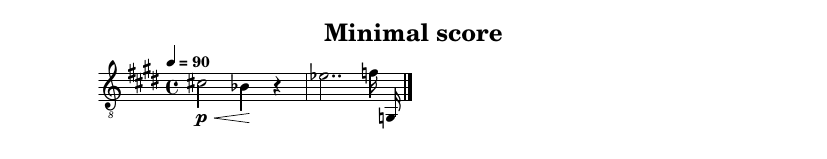
\includegraphics[scale=0.7]{../graphics/MinimalScore.png}

%    \vspace{0.25cm}

\begin{turn}{-1}
\maxsizebox{0.8\linewidth}{5cm}{
\begin{minipage}{\linewidth}
\begin{lstlisting}[language=CPlusPlus]
S_lpsrScore translateMsrToLpsr (
  S_msrScore          originalMsrScore,
  S_msrOahGroup       msrOpts,
  S_lpsrOahGroup      lpsrOpts,
  string              passNumber,
  string              passDescription,
  S_mfcMultiComponent multiComponent)
{
	// ... ... ...

  // create an msr2lpsrTranslator
  msr2lpsrTranslator
    translator (
      originalMsrScore);

  // build the LPSR score
  S_lpsrScore
    resultingLpsr =
      translator.translateMsrToLpsr (
        originalMsrScore,
        multiComponent);

	// ... ... ...

  return resultingLpsr;
}\end{lstlisting} % no line break here
\end{minipage}
}
\end{turn}

  \vfill

  \end{center}
\end{titlepage}


% -------------------------------------------------------------------------
{ % reduce vertical size of tables and lists
  \setlength {\parskip} {0.3ex plus \baselineskip minus 2pt}

  \tableofcontents

  \listoffigures
}


%% -------------------------------------------------------------------------
%\part{Acknowledgements}
%% -------------------------------------------------------------------------

\newpage

\subimport{./}{acknowledgements}


% -------------------------------------------------------------------------
\part{MusicFormats API principles}
% -------------------------------------------------------------------------

\subimport{./}{APIPrinciples.tex}


% -------------------------------------------------------------------------
\part{The MXSR API}
% -------------------------------------------------------------------------

% now we can switch to the regular headers and footers
\useRegularPagesHeadersAndFooters


\subimport{./}{creatingScoresWithTheMxsrAPI.tex}


% -------------------------------------------------------------------------
\part{The MSR API}
% -------------------------------------------------------------------------

\subimport{./}{creatingScoresWithTheMSRAPI.tex}


% -------------------------------------------------------------------------
\part{The LPSR API}
% -------------------------------------------------------------------------

\subimport{./}{creatingScoresWithTheLPSRAPI.tex}


% -------------------------------------------------------------------------
\part{The BSR API}
% -------------------------------------------------------------------------


\subimport{./}{creatingScoresWithTheBSRAPI.tex}


% -------------------------------------------------------------------------
% postamble
% -------------------------------------------------------------------------

% -------------------------------------------------------------------------
\part{Indexes}
% -------------------------------------------------------------------------

% back to the lists fancyhead headers and footers
\useListsPagesHeadersAndFooters

\printindex[Files]

\printindex[Options]

\printindex[MusicXML]

\printindex[Main]


% -------------------------------------------------------------------------
\end{document}
% -------------------------------------------------------------------------
